\chapter{The Indexing}

\vspace{1em}
\hfill
\begin{minipage}[c]{0.55\textwidth}
\raggedleft
\small\itshape
The actual science of logic is conversant at present only with things either certain, impossible, or entirely doubtful, none of which (fortunately) we have to reason on. Therefore the true logic for this world is the calculus of probabilities.\\[0.5em]
\upshape\footnotesize James Clerk Maxwell, 1850
\end{minipage}%
\hspace{0.5em}
\begin{minipage}[c]{0.12\textwidth}
% \includegraphics[width=\textwidth]{figures/ch03_indexing.png}
\end{minipage}
\vspace{1.5em}

\noindent Chapter 2 ended with a name. Probability is the indexing procedure. You have been performing it your whole life, the way you perform induction: without thinking about it, often well, sometimes badly.

This chapter is about what probability actually is.

\section*{The structure of belief}

Probability is not a special science about gambling or radioactive decay. It is the structure of how you update beliefs in the face of evidence.

You hold beliefs with degrees. You are more confident that the sun will rise tomorrow than that your favorite team will win on Sunday. You are more confident that there is coffee in the cup in front of you than that the recipe in your head will taste right when you make it. Each belief is held with a strength that responds to evidence. A weather forecast adjusts your beliefs about Saturday. A friend's text changes your beliefs about what they think. The movement is not arbitrary. If you are a careful reasoner, the movement is determined by a rule.

The rule is the simplest thing in the world. It is counting.

\section*{Restriction}

The Library contains every possibility. You are somewhere in it. What does your data do?

It restricts you.

Before any data, every book in the Library is a candidate description of your situation. After data, only the books consistent with the data remain candidates. The set of consistent books is a subset of the Library. Your task, when you reason about which book is yours, is to point at which subset is correct, weighted by how plausible each member is.

This is the structure of conditional probability. Conditional probability is restriction to a subset, followed by counting within. Figure~\ref{fig:bayes-counting} shows the geometry.

\begin{figure}[h]
\centering
\begin{tikzpicture}[>=Stealth, scale=1.0]
  % Outer box (the Library)
  \draw[thick] (0,0) rectangle (10,5);
  \node[anchor=north east, font=\small\itshape] at (9.85,4.85) {the Library};

  % Circle H (hypothesis)
  \draw[thick, blue, fill=blue!15] (3.8,2.5) circle (1.7);
  \node[blue, anchor=south, font=\bfseries] at (2.5,3.7) {$H$};

  % Circle D (data) - overlapping, semi-transparent
  \draw[thick, red, fill=red!15, fill opacity=0.7] (6.2,2.5) circle (1.7);
  \node[red, anchor=south, font=\bfseries] at (7.5,3.7) {$D$};

  % Label in intersection
  \node[font=\small] at (5.0,2.5) {$H \cap D$};

  % Annotation
  \draw[->, gray] (8.6,0.6) -- (7.3,1.6);
  \node[gray, font=\scriptsize, anchor=west] at (8.5,0.4) {data restricts to $D$};
\end{tikzpicture}
\caption{Conditional probability as restriction. The outer rectangle is the Library: every possibility. The circle $D$ is the subset of cases consistent with what you have observed. The circle $H$ is the subset where the hypothesis you care about holds. The posterior $P(H \mid D)$ is the fraction of $D$ that also lies in $H$. Bayes' theorem is what you get when you write that fraction in terms of the original sizes.}
\label{fig:bayes-counting}
\end{figure}

In formula, the conditional probability of a hypothesis $H$ given data $D$ is

$$P(H \mid D) = \frac{|H \cap D|}{|D|}.$$

This is the definition. It is not a theorem. It is what the words mean: of the cases consistent with the data, what fraction also have the property?\footnote{For finite populations the counts are integers and the ratios are exact. For continuous or infinite possibility-spaces the counts become measures and the ratios are ratios of measures. The arithmetic is the same; the interpretation expands. Chapter 4 makes the measure question precise.}

Bayes' theorem is what you get when you rewrite this ratio. The numerator $|H \cap D|$ can be counted the other way around: among cases with $H$, the fraction that also have $D$ is $P(D \mid H)$. So

$$|H \cap D| = |H| \cdot P(D \mid H).$$

The denominator $|D|$ is the count of cases consistent with the data, split by whether $H$ holds:

$$|D| = |H| \cdot P(D \mid H) + |\neg H| \cdot P(D \mid \neg H).$$

Putting these together and dividing by the size of the Library to turn counts into probabilities:

$$P(H \mid D) = \frac{P(D \mid H) \, P(H)}{P(D \mid H) \, P(H) + P(D \mid \neg H) \, P(\neg H)}.$$

Or, more compactly,

$$P(H \mid D) = \frac{P(D \mid H) \, P(H)}{P(D)}.$$

This is Bayes' theorem. It is what counting in a restricted subset gives you.

The ``theorem'' is bookkeeping: it converts the count-in-a-subset definition into a calculation in terms of the original sizes. Every step is a rearrangement of the same count.

What the theorem does, restated: it asks how much of the data-consistent subset would come from each hypothesis, weighted by how common each hypothesis was in the original Library. Hypotheses that produce the data more often, and that were more plausible to begin with, dominate the restricted subset. Hypotheses that produce the data rarely, or that were implausible to begin with, fade. The proportions shift to match the evidence.

\section*{The coin}

The coin shows the counting in action.

Imagine ten thousand coin-flipping trials. Pick a fraction in which the coin is a trick coin, one that lands heads every time. Suppose trick coins are rare, so the fraction is one in a hundred: about $100$ trials are trick-coin trials, and about $9{,}900$ are fair-coin trials.

In each trial, the coin is flipped five times. Every trick-coin trial produces HHHHH. About $1/32$ of the fair-coin trials produce HHHHH, by chance. So the number of trials in the whole population that produce HHHHH is approximately

$$100 + \frac{9{,}900}{32} \approx 100 + 309 \approx 409.$$

Now restrict to those $409$ trials. Of those, $100$ are trick-coin trials and $309$ are fair-coin trials. The fraction of trick-coin trials within the restricted subset is

$$\frac{100}{409} \approx 0.244.$$

After five heads, the probability that the coin is a trick coin has jumped from $1\%$ to about $24\%$. Figure~\ref{fig:coin-counting} shows the populations before and after the restriction.

\begin{figure}[h]
\centering
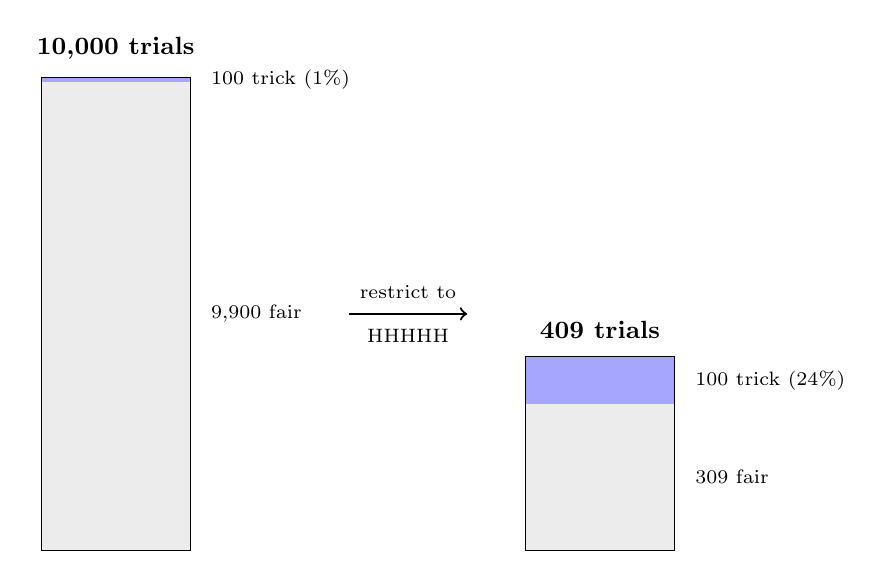
\begin{tikzpicture}[scale=0.75]
  % Left rectangle: prior population (10,000 trials), height 8 units
  \draw[thick] (0,0) rectangle (2.5,8);
  \fill[blue!35] (0,7.92) rectangle (2.5,8);
  \fill[gray!15] (0,0) rectangle (2.5,7.92);
  \node[anchor=south, font=\small\bfseries] at (1.25,8.15) {10{,}000 trials};
  \node[anchor=west, font=\scriptsize] at (2.7,7.96) {100 trick (1\%)};
  \node[anchor=west, font=\scriptsize] at (2.7,4) {9{,}900 fair};

  % Arrow
  \draw[->, thick] (5.2,4) -- (7.2,4);
  \node[anchor=south, font=\scriptsize] at (6.2,4.1) {restrict to};
  \node[anchor=north, font=\scriptsize] at (6.2,3.9) {HHHHH};

  % Right rectangle: restricted population (409 trials), height 3.27 units
  \draw[thick] (8.2,0) rectangle (10.7,3.27);
  \fill[blue!35] (8.2,2.47) rectangle (10.7,3.27);
  \fill[gray!15] (8.2,0) rectangle (10.7,2.47);
  \node[anchor=south, font=\small\bfseries] at (9.45,3.42) {409 trials};
  \node[anchor=west, font=\scriptsize] at (10.9,2.87) {100 trick (24\%)};
  \node[anchor=west, font=\scriptsize] at (10.9,1.24) {309 fair};
\end{tikzpicture}
\caption{The Bayesian update as counting. Left: the prior population of $10{,}000$ trials, $1\%$ trick coins (the thin blue band). Right: restricted to the $409$ trials that produced HHHHH. All $100$ trick-coin trials survive (every one produces HHHHH); only about $309$ of the $9{,}900$ fair-coin trials do. The shape of the population changes. Within the restriction, the trick fraction has grown from $1\%$ to about $24\%$, not because any individual trial changed, but because the data restricted the count.}
\label{fig:coin-counting}
\end{figure}

That is the entire Bayesian calculation. Counted, not derived. The formula of Bayes' theorem gives the same answer through different bookkeeping. The data did not prove anything. It restricted you to a subset, and within that subset, the proportions tell you what you should now believe.

\section*{The unique calculus}

You could in principle use other rules for combining degrees of belief. Many have been proposed. Almost none are consistent.

Consider what consistency rules out. Suppose your rule combines two pieces of evidence by adding their strengths instead of multiplying likelihoods. You see one piece of evidence that supports $H$ to degree $0.6$. You see a second, independent piece, also supporting $H$ to degree $0.6$. Adding gives $1.2$. But a degree of belief should be bounded by certainty; it cannot exceed $1$. The rule produces nonsense at the edges, which means it is producing nonsense in proportion everywhere short of the edges.

Or suppose your rule gives different posteriors depending on the order in which evidence arrives. You see $D_1$ and then $D_2$ and conclude $P(H) = 0.8$. You see $D_2$ and then $D_1$ and conclude $P(H) = 0.6$. The evidence is the same. A consistent agent should reach the same conclusion either way; the order in which two pages of a letter are read should not change what the letter says.

In 1946, the physicist R.\ T.\ Cox proved that the rules required to avoid these and similar pathologies, taken together, force your calculus to be (isomorphic to) probability theory.\footnote{Cox required only modest consistency desiderata: degrees of belief are real numbers; two paths to the same conclusion give the same answer; the calculus reduces to classical logic in the limit of certainty. The original proof has loose ends that have been tightened by later authors, but the conclusion is robust.} The desiderata are short and hard to argue against. The conclusion is that Bayesian updating is the unique calculus of belief that does not contradict itself.

This means any agent that is internally consistent, that does not contradict itself in repeated applications, and that respects classical logic where logic suffices, is doing Bayesian inference. Whether they know it or not. Whether they have read this chapter or not. Whether they call it Bayesian or not.

You have been doing this your whole life. The mathematics is just the explicit form.

\section*{The missing piece}

Bayes' theorem is precise. Cox's theorem says it is unique. Together they specify how you should update beliefs in the presence of evidence.

What they do not specify is where you should start.

The numbers in the coin example came from somewhere: a prior of $1\%$ for trick coins. Why that number? Because most coins are fair. But how do you know that? Past experience with coins. And past experience with coins gives you a probability over coins by, presumably, Bayesian updating. Which requires a prior over coins. Which had to come from somewhere.

The regress goes all the way down. Bayes tells you what to do once you have a prior. It does not tell you what the prior should be.

A reasonable agent could start with $P(\text{trick}) = 0.5$, treating fair and trick coins as equally likely. After five heads, they would be at about $0.97$.

Another reasonable agent could start with $P(\text{trick}) = 0.001$. After the same five heads, they would be at about $0.030$.

Both are using Bayes. Both are internally consistent. Both are answering the same question with the same data. They get different answers because they started in different places. Cox's theorem cannot adjudicate. Bayes' theorem cannot either. The choice of prior is, in the standard treatment, a matter of taste, of prior knowledge, or of guess.

This is the problem of induction returning, in a different form. Hume said there is no logical justification for inferring future from past. Bayes says: given a prior, here is how to do the inference. The hard question, the one that resists, is the same one. Where does the prior come from?

\section*{Where this leaves you}

You have a procedure for updating beliefs. The procedure is unique. It is also incomplete: it requires an input the procedure itself cannot supply.

For two and a half centuries, this gap was treated as a fact about the limits of pure reason. Priors are subjective. They reflect agent-specific commitments that mathematics cannot dictate. Different reasonable agents may end with different posteriors, and there is no principled way to declare one of them right.

That was the consensus until the 1960s.

The next chapter shows the prior is not, after all, free. The Library has a natural measure, and the measure is the prior. It comes from a counting argument on prefix-free codes that fits in one page.
